%Original Template by Everen Wegner
\documentclass{formalLabReport} %Change to informal to see other template
\urlstyle{same}

%Declare Package Usage
\usepackage{siunitx}
\usepackage{todonotes}
\usepackage[table,xcdraw]{xcolor}
\usepackage{pdflscape}
\usepackage{attachfile}
\usepackage[paper=A4]{typearea}
\usepackage{tikz}
\usetikzlibrary{snakes}
\usepackage{listings}


%Title Page
\title{SPA4a}
\author{Andy Dao, Helina Mulugeta}
\prof{Professor Khan}
\className{Procedural and Object Oriented C++}
\classCode{CSC 2210 001}
\submissionDate{10/29/2024}
\githubRepo{https://github.com/ViviVoid/daoa-mulugetah-spa4/tree/main} 
%For Informal Reports
\laboratoryDate{01/17/2024} % Submission Date


\lfoot{\footnotesize{}}

\begin{document}

% 1. Title Page
% a. Student Names
% b. Date
% c. Assignment Title
% d. Repository Link (linkable preferred)
\maketitle
% \tableofcontents
% \listoffigures
% \newpage

\section{The Dungeon}

You are in a dungeon with 25 rooms, hunting for the Wumpus. 

\subsection{Hazards}
Two dragons roam the dungeon and if they find you, they will relocate you to a random room in the dungeon. When you are next to a room with dragons, you will smell a "scent of charcoal".

There are two pit traps and if you enter their room, you will fall to your death. When you are next to a room with a pit trap, you will hear "echoes of water drops".

Your goal is to unlock the cage the Wumpus is in by collecting the three gems located in various rooms in the dungeon that will force thet the gates open. Once open, you need to find the room the Wumpus is in and capture it. You have a few nets that you came prepared with. In case you miss the Wumpus when throwing to catch it, you will find some more around the dungeon. If the room the Wumpus is in is unlocked, you will  "hear slight shuffling."

Although the odds are against you, you may find a trusty lantern to help you along the way. If found, the lantern will show what is ahead in a room of your choice. Careful though, you can only use the lantern three times before it runs out of fuel.

Action: 
\begin{itemize}
    \item \textbf{N})orth
    \item \textbf{S})outh
    \item \textbf{E})ast
    \item \textbf{W})est
    \item attempt \textbf{C})apture
    \item \textbf{L})antern
    \item display \textbf{I})nventory
    \item \textbf{H})elp
    \item \textbf{Q})uit
\end{itemize}

\newpage

\section{Implementation Specifics}
\subsection{Andy Dao}

Interactables and all inheriting classes shall be implemented by Andy Dao.

\subsection{Helina Mulugeta}

Dungeon, Room and Player classes shall be implemented by Helina.\newline

\section{Sample Map}

\begin{verbatim}
? + . . >
. @ . ! .
. g > g ?
> . @ # .
g ! . . @
\end{verbatim}

\begin{itemize}
    \item + : Player
    \item \# : Wumpus
    \item ? : Lantern
    \item > : Nets
    \item $@$ : Pit Traps
    \item ! : Dragons
    \item g : Gems
\end{itemize}

\begin{figure}
    \centering
    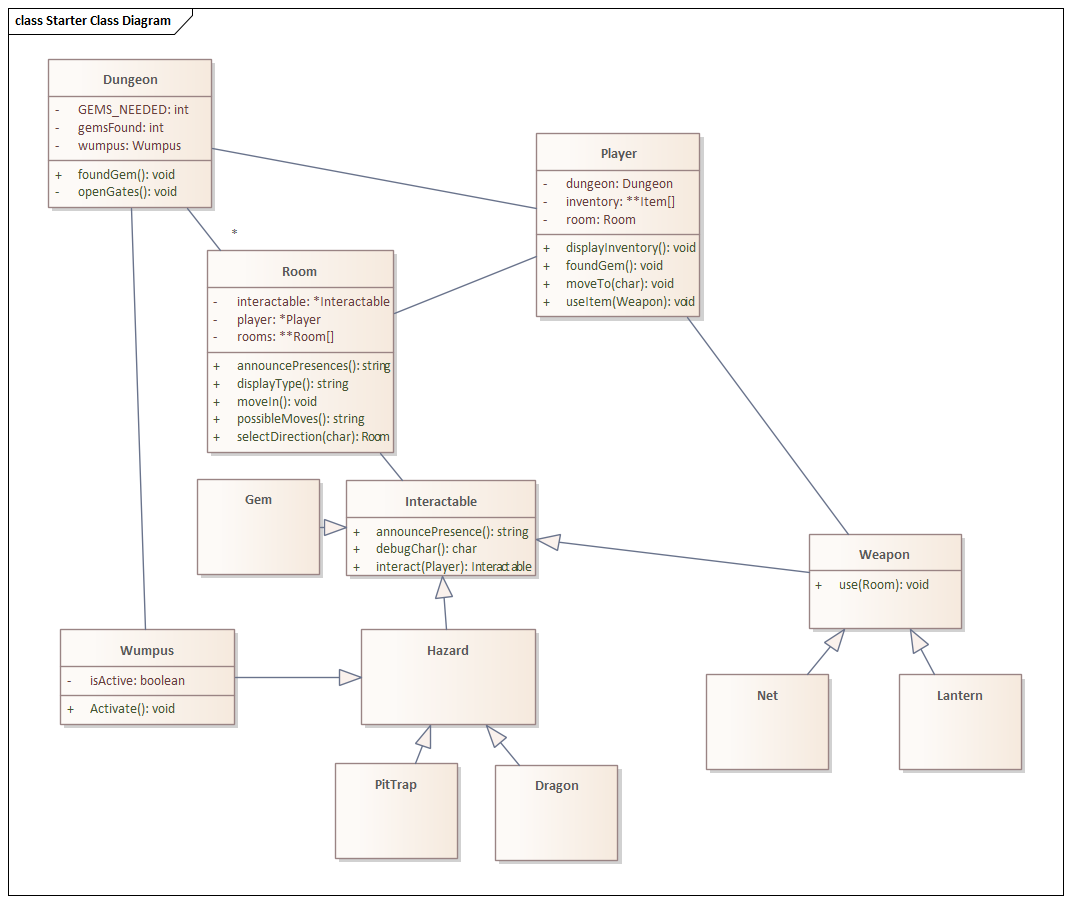
\includegraphics[width=1\linewidth]{Class Diagram.png}
    \caption{Class Diagram}
    \label{fig:enter-label}
\end{figure}

\section{Uniqueness}

Our version of Hunt the Wumpus has a lantern which will provide the player additional clues if found. This gives the player the incentive to move to various rooms and find lanterns but still limits them from overusing since they are limited to 3 uses. There are also gems that the player needs to collect before the Wumpus can be released. This will give the player time to get accustomed to moving around the map before they can start hunting the Wumpus. This is not without danger though, as they can still fall into a pit. 



\end{document}